\documentclass[12pt,a4]{article}

\usepackage{amsfonts}
\usepackage[T1]{fontenc}
\usepackage[utf8]{inputenc}
\usepackage{amsmath}
\usepackage{graphicx}

\title{Use case sfide}
\begin{document}
\maketitle
In questo documento verrà mostrato il modo in cui si svolgeranno le sfide tra utenti nell'applicazione. Nelle varie sezioni verranno indicati gli attori delle operazioni, gli elementi del progetto coinvolti e i messaggi scambiati dagli stessi.

\section*{Use case}
Nell'analisi riguardo le sfide tra gli utenti sono stati individuati i casi d'uso descritti in seguito nel documento.\\
\\Sono stati individuati due attori principali che interagiscono con il sistema:
\begin{itemize}
\item Sfidante: il giocatore che inizia il processo di sfida
\item Giocatore sfidato: il giocatore che riceve la sfida
\end{itemize}
La comunicazione tra i due attori è mediata dalle loro relative applicazioni che comunicano attraverso il Server. 
\subsection*{Selezione dello sfidante}
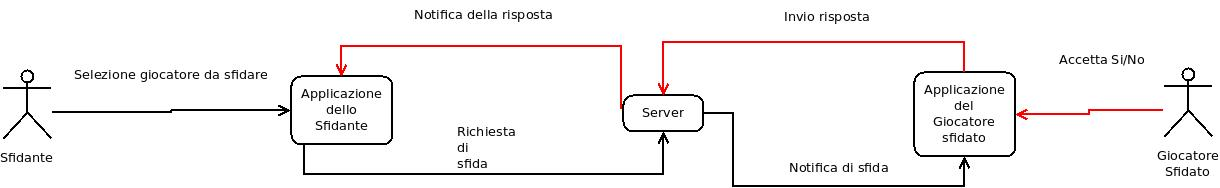
\includegraphics[scale=0.3]{./UseCaseSfide.jpeg}\\
Il giocatore che volesse iniziare una sfida con un altro utente diventa lo Sfidante. Questi si troverà inizialmente sulla schermata in cui è mostrata la mappa con tutti i giocatori attivi nelle vicinanze. Lo Sfidante seleziona un giocatore sulla mappa che diventa il Giocatore sfidato.\\

\textbf{Azioni svolte dagli attori:}
\begin{itemize} 
\item Sfidante(Selezione del giocatore): lo Sfidante seleziona sulla mappa il giocatore da sfidare
\item ApplicazioneSfidante(Richiesta di sfida): invia al Server la richiesta di sfida e attende la risposta mostrando allo Sfidante una schermata d'attesa. Se la risposta non arriva dopo 10 secondi la sfida viene annullata.
\item Server(Notifica di sfida): invia all'ApplicazioneGiocatoreSfidato la notifica per cui lo sfidante vuole iniziare una sfida.
\item GiocatoreSfidato(Risposta): il GiocatoreSfidato, ricevuta la notifica, seleziona nella schermata apposita la risposta. La risposta viene inviata al Server. Se la risposta è positiva attende per 10 secondi l'inizio della sfida, in ogni altro caso la sfida termina.
\item Server(Notifica della Risposta): invia all'applicazione dello Sfidante la risposta del GiocatoreSfidato il quale in caso di risposta affermativa inizia la sfida.
\end{itemize}

\subsection*{Svolgimento della sfida}
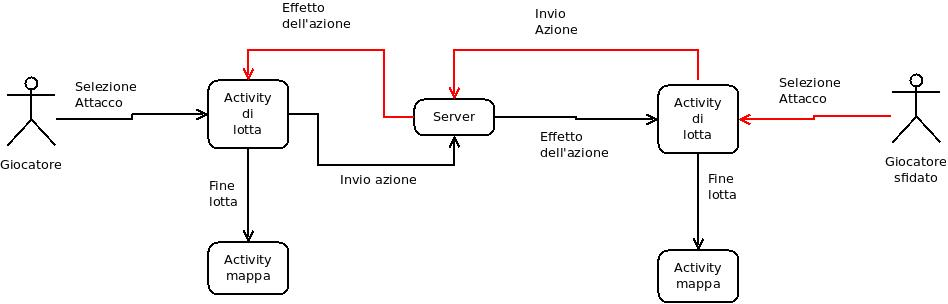
\includegraphics[scale=0.4]{./UseCaseSvolgimentoLotta.jpeg}\\
Una volta concluso il processo di selezione dello sfidante inizia la sfida. La sfida si svolge a turni. Entrambi i giocatori sono riportati alla schermata di lotta e il primo turno è dello Sfidante. Ogni giocatore al proprio turno seleziona l'azione da eseguire.\\
\\
\textbf{Azioni svolte dagli attori:}
\begin{itemize}
\item Sfidante(Selezione dell' Attacco): seleziona un'azione disponibile al momento.
\item ApplicazioneSfidante(InvioAzione): invia al Server l'azione da effettuare cedendo il turno all'avversario
\item Server(Effetto dell'azione): comunica all'ApplicazioneGiocatoreSfidato l'inizio del turno del GiocatoreSfidato con l'azione dello sfidante.
\item GiocatoreSfidato: le sue azioni sono le stesse dello sfidante
\end{itemize}
La lotta termina quando la vita di uno dei due giocatori viene ridotta a 0 il quale perderà la sfida. Ad entrambi viene mostrato il riepilogo della lotta e infine riportati sulla mappa di gioco.
\end{document}